\documentclass[a4paper,12pt,answers]{exam}
\usepackage{graphicx} % Required for inserting images
\graphicspath{ {images/} }
\usepackage{amsmath}
\usepackage{amssymb}

\title{CS215 Assignment-1}
\author{Malay Kedia, Aakash Gupta, Yash Singh}
\date{August 2024}

\begin{document}
\maketitle
\begin{questions}
\question{\bf Fitting Data}\\
\textbf{Task B}
\begin{solution}\\
    Graphically the the normal distribution parameter $\mu$ seems to be around 6.
\begin{center}
    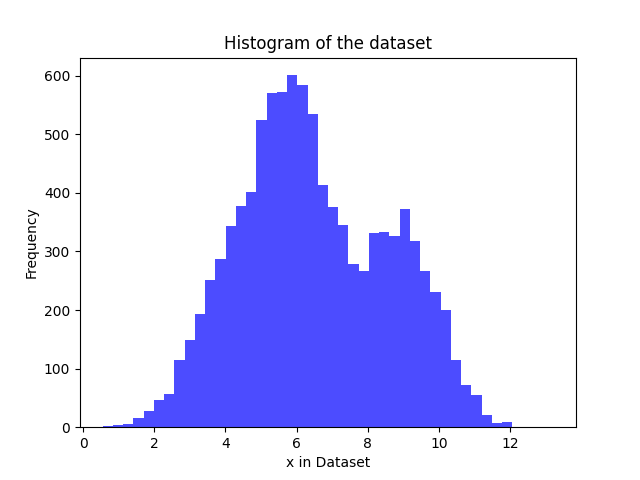
\includegraphics[width=0.75\linewidth]{3b.png}
    \caption{\\Histogram plot}
\end{center}
\end{solution}
\textbf{Task C}
\begin{solution}\\
Let $X \sim Bin(n,p)$\\
First moment of Binomial Distribution, $\mu_{1}^{bin}$
\[\mu_{1}^{bin} = E(X) = \sum_{x=0}^{n} x \binom{n}{x} p^x (1-p)^{n-x} \]
\[\mu_{1}^{bin}= np \sum_{x=1}^{n} \binom{n-1}{x-1} p^{x-1} (1-p)^{n-x} \]
\[\mu_{1}^{bin}= np (1-p + p)^{n-1}\]
\[\mu_{1}^{bin}= np\]
Second moment of Binomial Distribution, $\mu_{2}^{bin}$
\[\mu_{2}^{bin} = E(X^2) = \sum_{x=0}^{n} x^2 \binom{n}{x} p^x (1-p)^{n-x} \]
\[\mu_{2}^{bin}= \sum_{x=0}^{n} \left\{x(x-1) + x\right\} \binom{n}{x} \binom{n-1}{x-1} \binom{n-2}{x-2} p^x (1-p)^{n-x} \]
\[\mu_{2}^{bin}= n(n-1)p^2 \left\{\sum_{x=2}^{n} \binom{n-2}{x-2} p^{x-2} (1-p)^{n-x}\right\} + np \]
\[\mu_{2}^{bin}= n(n-1)p^2 (1-p + p)^{n-2} + np \]
\[\mu_{2}^{bin}= n(n-1)p^2 + np\]
\[\mu_{2}^{bin}= np(1-p) + n^2 p^2\]
\begin{center}
    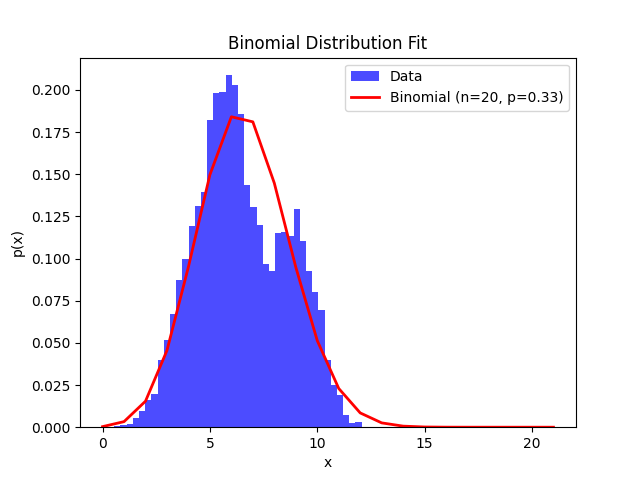
\includegraphics[width=0.75\linewidth]{3c.png}
    \caption{\\Binomial Fitting}
\end{center}
\end{solution}
\textbf{Task D}
\begin{solution}\\
Lets calculate $i^{th}$ moment of gamma function given by:
\[
f(x,\alpha,\theta) = \frac{x^{\alpha - 1} }{\Gamma(\alpha)\theta^{\alpha}} e^{-\frac{x}{\theta}}
\]
\[E[X^i] = \int_{0}^{\infty} \frac{ x^k}{\Gamma(\alpha)\theta^{\alpha}} x^{\alpha - 1} e^{-\frac{x}{\theta}} \, dx 
= \frac{1}{\Gamma(\alpha)\theta^{\alpha}} \int_{0}^{\infty} x^{(\alpha + i) - 1} e^{-\frac{x}{\theta}} \, dx\]

\[= \frac{\Gamma(\alpha + i)\theta^{\alpha + i}}{\Gamma(\alpha)\theta^{\alpha}} \cdot \int_{0}^{\infty} \frac{1}{\Gamma(\alpha + i)\theta^{\alpha+i}} x^{\alpha + i - 1} e^{- \frac{x}{\theta}} \, dx \]

\[= \frac{\Gamma(\alpha + i)\theta^{\alpha + i}}{\Gamma(\alpha)\theta^{\alpha}} \cdot
\quad \text{(p.d.f. of } \Gamma(\alpha + i, \theta) \text{ integrates to 1)}\]

\[= \frac{\Gamma(\alpha + i)\theta^{\alpha + i}}{\Gamma(\alpha)\theta^{\alpha}}
= \frac{\theta^{i}\Gamma(\alpha + i)}{\Gamma(\alpha)} \]

\[= \frac{\theta^{i}(\alpha + i - 1)(\alpha + i - 2) \cdots \alpha \Gamma(\alpha)}{\Gamma(\alpha)} 
= \theta^{i}(\alpha + i - 1) \cdots \alpha.\]
Thus,\\
First moment $\mu_{1}^{gamma}$ is given by (replacing $\alpha$ by k in above derivation),\\
\[\mu_{1}^{gamma}=k\theta\]
And second moment $\mu_{2}^{gamma}$ is given by,\\
\[\mu_{2}^{gamma}=k(k+1)\theta^{2}\]
\begin{center}
    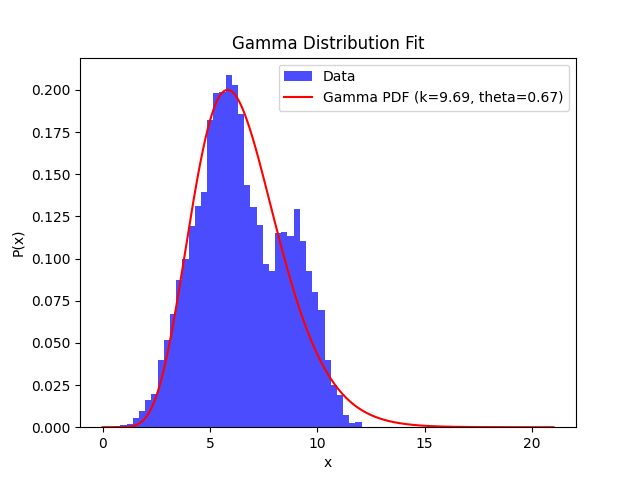
\includegraphics[width=0.75\linewidth]{3d.png}
    \caption{\\Gamma Fitting}
\end{center}
\end{solution}
\textbf{Task E}
\begin{solution}\\
    The likelihood of binomial (-2.1570681154346776) is a bit greater (closer to zero ) than likelihood of gamma distribution (-2.1608217722067953) indicating that binomial is a better fit.
\end{solution}
\textbf{Task F}
\begin{solution}\\
    The likelihood of  Mix Guassian distribution obtained is -2.183038744911319. This however is not better than any of the previous two!!
\begin{center}
    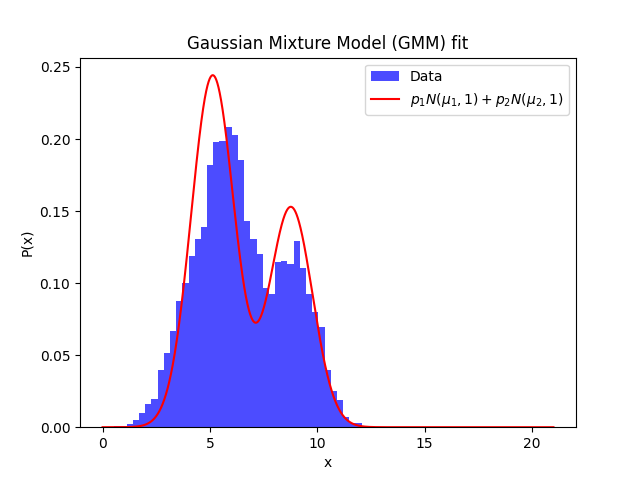
\includegraphics[width=0.75\linewidth]{3f.png}
    \caption{\\GMM Fitting}
\end{center}
\end{solution}
\textbf{Ungraded Bonus Question}
\begin{solution}\\
    In order to get a better fit, lets choose again a mixture of guassian distribution. The difference from previous case is that instead of two guassian, lets take three distribution superimposed over each other with probabilities p1, p2 and p3, mean as $\mu1$, $\mu2$ and $\mu3$ and variance of all of them as 1.\\
    The two new moments (fifth and sixth) can be derived giving the following expression:\\
    \[
     moment5^{th}=\mu ^{5}+10\mu ^{3}\sigma ^{2}+15\mu \sigma ^{4}
    \]
    \[
    moment6^{th} = \mu ^{6}+15\mu ^{4}\sigma ^{2}+45\mu ^{2}\sigma ^{4}+15\sigma ^{6}
    \]
    Similar to the previous method, calculating $5^{th}$ and $6^{th}$ moment of given dataset and solving the equations using fsolve fucntion of scipy, we were getting impossible soltions as the jacobian failed to converge.\\
    Thus making an initial guess and hypertuning the probabilities of the GMM, we finally arrived at a better fit whose GMM is as follows:
    \[
    Y \thicksim p1\cdot N_{1}(\mu1,1) + p2\cdot N_{2}(\mu2,1) + p3\cdot N_{3}(\mu3,1)
    \]
    \newline
    \[
    where,\\
    p1=0.5018740341610936\]
    \[\mu1=6.02960769428528\]
    \[p2= 0.2996456511927248\]
    \[\mu2=9.07436305441652\]
    \[p3= 0.200116472923\]
    \[\mu3=4.1000265473
    \]
    Thus the final fit is:
    \begin{center}
    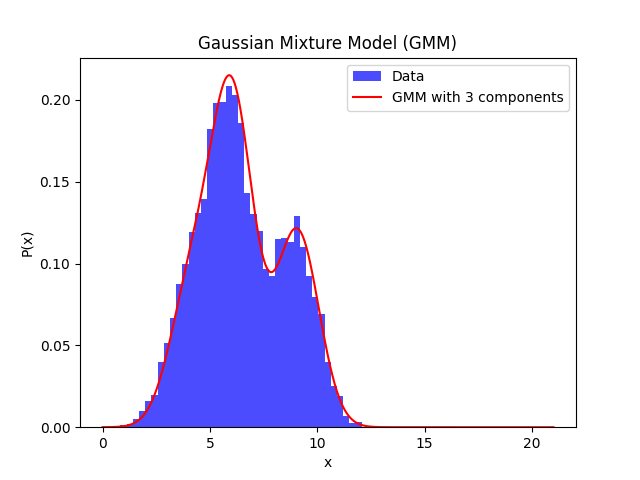
\includegraphics[width=0.75\linewidth]{3bonus.png}
    \caption{\\Final GMM Fitting}
\end{center}
\end{solution}
\end{questions}
\end{document}
